\documentclass[10pt]{article}
\usepackage{amscd,amsfonts,amssymb,amstext,latexsym} 
\usepackage{amsmath,mathbbol,mathrsfs,stmaryrd, mathtools} 

%\usepackage{mathbbol,mathrsfs,stmaryrd}
\usepackage {algorithm} 
\usepackage{theoremref}
\usepackage[T1]{fontenc}
\usepackage[english]{babel} 
\usepackage {enumerate}
\usepackage{url}
\usepackage[noend]{algpseudocode}
\usepackage{float}
\usepackage{graphics} 
\usepackage{tikz}
\usepackage[width=14.8cm,left=3cm,margin=1in]{geometry}
\usetikzlibrary{automata,calc}
%\usepackage{tgtermes} 
\usepackage{listings}
\usepackage{mathptmx}
\usepackage{fancyhdr}
\usepackage{verbatim}
\usepackage{enumitem}
\usepackage{booktabs}
\usepackage[flushleft]{threeparttable}
\usepackage{listings}
\usepackage{verbatim}
\usepackage{fancyhdr}
\usepackage{multirow,multicol}
\usepackage{color}
\usepackage[toc,page]{appendix}

\usepackage[utf8]{inputenc}
\usepackage{graphicx}


\usepackage[colorlinks=true,linkcolor=blue,citecolor=blue,urlcolor=blue]{hyperref}
\usepackage{tabto}
\lstset{ %
language=C,                % choose the language of the code
basicstyle={\ttfamily},       % the size of the fonts that are used for the code
backgroundcolor=\color{white},  % choose the background color. You must add \usepackage{color}
showspaces=false,               % show spaces adding particular underscores
aboveskip=6mm, 
%belowskip=3mm, 
numbers=left, numberfirstline=false, numberblanklines=false,
numberstyle=\tiny\color{gray}, numbersep= 5pt, 
showstringspaces=false,         % underline spaces within strings
showtabs=false,                 % show tabs within strings adding particular underscores
%frame=single,           % adds a frame around the code
%frame = tb, 
frame = none, 
tabsize=2,          % sets default tabsize to 2 spaces
captionpos=b,           % sets the caption-position to bottom
breaklines=true,        % sets automatic line breaking
breakatwhitespace=false,    % sets if automatic breaks should only happen at whitespace
escapeinside={\%*}{*)}          % if you want to add a comment within your code
}
%\graphicspath{{../../pics/}}
\fancypagestyle{plain}{
\fancyhf{}
\rhead{School of Computer Science and Applied Mathematics\\ 
%\noindent\rule{15.4cm}{0.4pt}\\
\footnotesize{\textsc{University of the Witwatersrand, Johannesburg}}}
\lhead{
\includegraphics[scale=0.08]{witslogo_h.png}}
\fancyfoot[C]{\thepage}
\renewcommand{\headrulewidth}{0.4pt}
}

%\textwidth=16.8cm 
%\textheight=22.6cm 
\evensidemargin 0pt 
\oddsidemargin 0pt 
\leftmargin 0pt 
\rightmargin 0pt 
\setlength{\topmargin}{0pt} 
\setlength{\footskip}{50pt}
\setlength{\parindent}{0pt}
\setlength{\parskip}{0.5em}
\linespread{1} 
% 
\makeatletter
\newcommand{\rmnum}[1]{\romannumeral #1}
\newcommand{\Rmnum}[1]{\expandafter\@slowromancap\romannumeral #1@}
\makeatother

%Custom commands for logical operators and other pseudocode stuff
\algnewcommand\AND{\textbf{ and }}
\algnewcommand\OR{\textbf{ or }}
\algnewcommand\NOT{\textbf{not}}
\algnewcommand\BREAK{\textbf{break}}
\algnewcommand\RETURN{\textbf{return }}

\begin{document}
\title{COMS4040A Assignment 1 -- Report}
\author{Tamlin Love (1438243) - BSc Hons}
\date{\today} 
\maketitle 
%\thispagestyle{empty}
\pagestyle{fancy}
\fancyhf{}
\fancyhead[R]{\thepage}
\fancyhead[L]{COMS4040A Assignment 1}
%\vskip 3mm 
%\pagenumbering{roman}
%\newpage
\pagenumbering{arabic} 
\vspace{-1.5cm}
\section{Introduction}\label{Introduction}
The k nearest neighbour (KNN) algorithm is a simple, widely used algorithm in used for classification and regression problems\cite{altman92}. Its applications vary from detecting intrusive programs\cite{liao02} to text classification \cite{kwon03} to the analysis of nuclear magnetic resonance spectra \cite{kowalski72}.
\\
The algorithm itself is very simple. Consider a set $P$ of $m$ reference points $p_{i}\in\mathbb{R}^{d}$ and a set $Q$ of $n$ query points $q_{j} \in \mathbb{R}^{d}$. The aim of the algorithm is to find the $k$ nearest (according to some distance measure) points in $P$ for each $q_{j}\in Q$, for some integer $k$.
\\
In the brute force approach we first compute the distance between each query point and each reference point and store it in a distance matrix of size $n \times m$. We then sort each row in the matrix before returning the $n \times k$ (keeping track of any swaps via the index matrix), before returning the $n \times k$ index sub-matrix containing the indices of the k-nearest neighbours to each query point.
\\
Special attention must be given to the distance measure and sorting functions applied above. In this report, we consider the Euclidean and Manhattan distance measures, and for sorting we consider the quicksort, bubblesort and mergesort algorithms.
\\
Because any distance measure in $\mathbb{R}^{d}$ must take $\mathcal{O}(d)$ time to compute, the k nearest neighbours algorithm must take $\mathcal{O}(mnd)$ time to compute distances. Since quicksort and mergesort are both $\mathcal{O}(mlog(m))$ on average, and bubblesort is $\mathcal{O}(m^2)$ on average, the final algorithm must take $\mathcal{O}(nmlog(m))$ time to sort using quicksort or mergesort, and $\mathcal{O}(nm^2)$ time to sort using bubblesort. For large $m$, $n$ and $d$, these complexities are problematic. However, as we shall see in Section \ref{Methodology}, this can be significantly improved upon using parallel algorithms.
\section{Methodology}\label{Methodology}
As mentioned in Section \ref{Introduction}, there are two computationally intensive sections in the algorithm: the distance computation and the sorting component. We shall apply Foster's Design Methodology to each of these sections individually in the hope of improving the performance of the algorithm.
\subsection{Distance Computation}
Consider the two distance measures. Because the only difference between these algorithms is the square of the difference in the Eucidean metric and the absolute value of the difference in the Manhattan metric, they can be dealt with in the same way. No matter the algorithm used, the distance function is performed $nm$ times in the k nearest neighbours algorithm. Furthermore, the computation of the distance between points $q_{i}$ and $p_{j}$ is in no way dependent on the computation of distance between points $q_{s}$ and $p_{t}$ for $s\neq i$ and $t\neq j$. We will therefore collapse the for-loops in the algorithm which iterate over each  $q_{i}$ and $p_{j}$ into $nm$ tasks which can be divided among processors. 
\\
In practice, this partitioning is done by the OpenMP \textbf{for} directive with the \textbf{collapse(2)} clause. The communication, agglomeration and mapping steps are performed by the OpenMP compiler.
\subsection{Sorting}
Consider the sorting algorithms. These are all repeated $n$ times, once for each $q_{i}$. Here, rather than focus on the loop over each $i$, we will focus on applying Foster's Design Methodology to each sorting algorithm individually.
\paragraph{Quicksort:}
Here we note that each call to Quicksort recursively calls Quicksort on two portions of the list. We can therefore partition each recursive call into a separate task to be executed by a thread. This is done using the OpenMP \textbf{sections}/\textbf{section} construct. However, at a certain point, the overhead involved with scheduling threads becomes significant, so that sorting a small sublist in serial is actually faster than further partitioning the task. We therefore introduce a condition: if $high-low<c$ for some cut-off $c$, we will sort in serial. Otherwise, we will partition further. Communication, agglomeration and mapping is then handled by the OpenMP compiler.
\paragraph{Mergesort:}
Here we note that Mergesort, like Quicksort, recursively calls Mergesort on two portions of the list. Therefore, we can parallelisze it identically: by partitioning each recursive call into a separate task using the OpenMP \textbf{sections}/\textbf{section} construct. Once again, we employ the cut-off condition to reduce overhead.
\paragraph{Bubblesort:}
Here we employ an algorithm known as the Odd-Even sort or the Parallel-Neighbour sort \cite{habermann72}, which essentially sorts pairs of numbers in the list in parallel. These pairs alternate from 0-1, 2-3, 4-5, etc. (even) to 1-2, 3-4, 5-6, etc. (odd). This can be thought of as the parallel version of the bubblesort.
\\
In this algorithm we partition each inner for-loop into a task using the OpenMP \textbf{for} directive. Once again, communication, agglomeration and mapping are handled by the OpenMP compiler.
\section{Empirical Analysis}
The following experiments were run on XXX with 4 cores and, therefore, 4 threads were used. Random points in $\mathbb{R}^{d}$ using the \textit{generatePoints.py} file and stored in text files which were read in by the programs. For each experiment, the time taken to calculate every distance and the time taken to sort every list were measured and tabulated. Thus the total time is comprised only of these two measures.
\\
In the first experiment, $n$ varied between $n = 200$, $n = 800$ and $n = 1600$, with constant $d = 32$ and $m = 1000$. All 3 sorting algorithms and both distance metrics are used in the serial and parallel (using OpenMP \textbf{sections} construct) approaches. The results are tabulated below.
\begin{figure}[H]
\caption{$d = 32$, $m = 1000$}
\centering
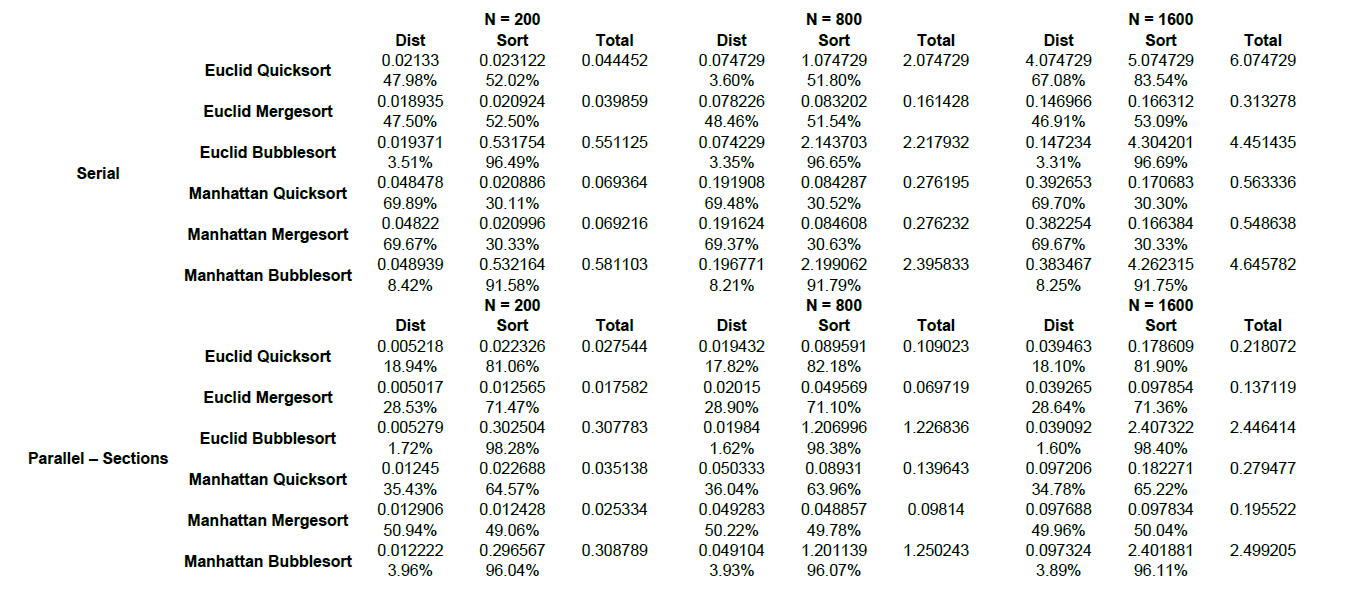
\includegraphics[scale=0.5]{d32m1000.png}
\end{figure}
What is immediately clear is that bubblesort is by far the slowest of the sorting algorithms, in both serial and parallel. Mergesort is on average slightly faster than quicksort in serial, and noticeably faster than quicksort in parallel. Overall, the parallel approach is much faster, with quicksort being 1.77 times as fast, bubblesort being 1.85 times as fast and mergesort being 2.59 times as fast. What is also clear is that the Euclidean distance metric is, on average, faster than the Manhattan metric, in both approaches.
\\
Consider now the same experiment with $m=10 000$.
\begin{figure}[H]
\caption{$d = 32$, $m = 10000$}
\centering
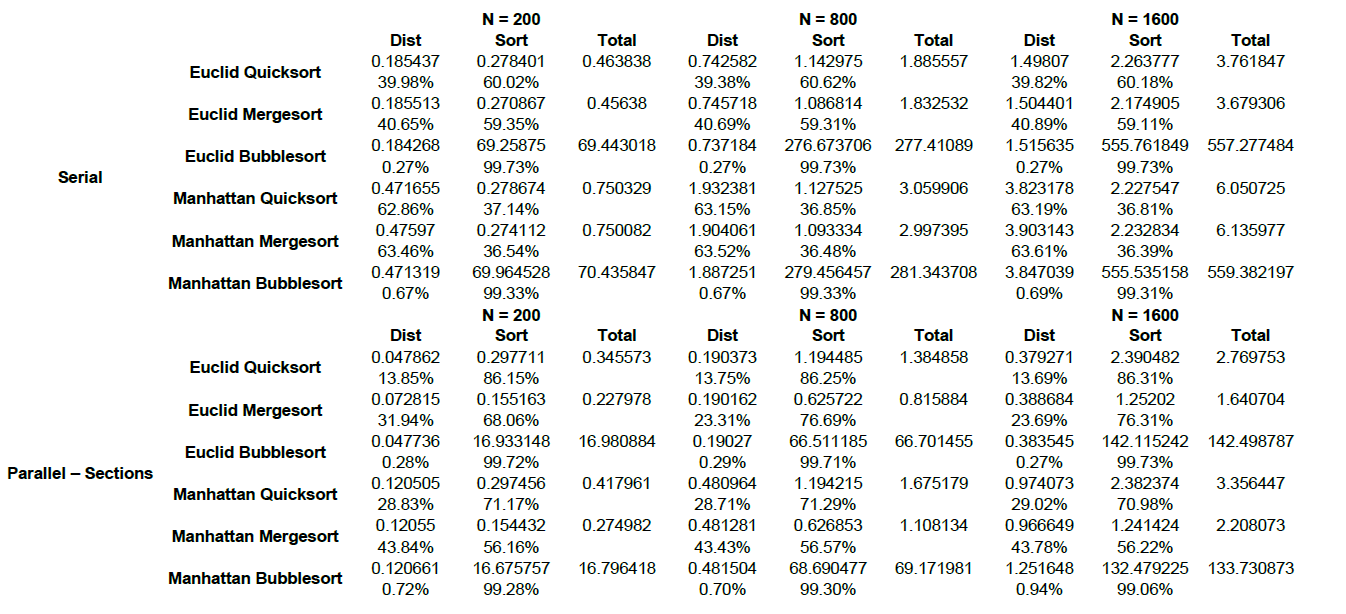
\includegraphics[scale=0.5]{d32m10000.png}
\end{figure}
Here it is even more clear that the bubblesort is inefficient, as its time complexity scales quadratically in $m$. With such a large $m$, the advantages of the parallel approach are even more apparent, with quicksort speeding up by a factor of 1.61, mergesort by 2.53 and bubblesort by 4.07.
\\
We now vary $d = 64, 128, 256, 512$ and keep $n=800$, $m=5000$ constant. For brevity's sake, we consider only the quicksort algorithm.
\begin{figure}[H]
\caption{$n=800$, $m=5000$}
\centering
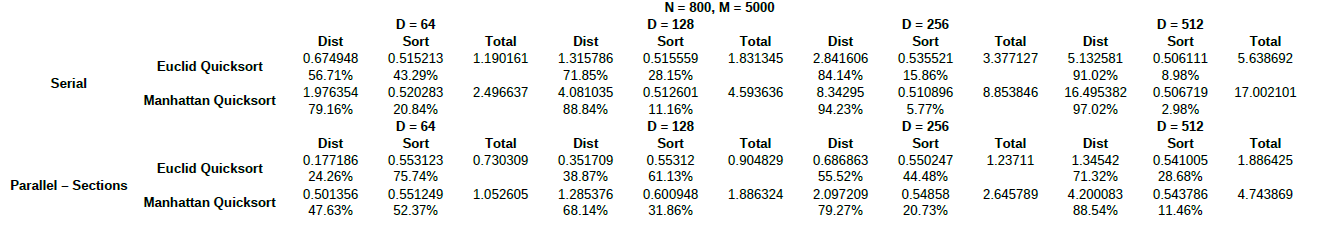
\includegraphics[width=\textwidth]{n800m5000.png}
\end{figure}
Here it is easily observed that the Manhattan metric is much slower than the Euclidean one. This is likely due to the presence of a conditional statement when evaluating $|p_{i}-q_{i}|$. We also note the effectiveness of the parallelisation, which on average sped the Euclidean calculation by a factor of 2.74 and the Manhattan calculation by a factor of 3.19.
\section{Summary}
\bibliographystyle{IEEEannot}
\bibliography{myBib}
\begin{comment}
\begin{appendices}
\section{Algorithms}\label{app:Algorithms}
\begin{algorithm}[H]
\caption{k Nearest Neighbour}\label{alg:kNN}
\begin{algorithmic}[1]
\Procedure{kNN}{P,Q,k}
	\State distance $\gets [][]$
	\State index $\gets [][]$
	\For{$q_{i}\in Q$}
		\For{$p_{j} \in P$}
			\State distance[$i$][$j$] $\gets$ dist($q_{i},p_{j}$)
			\State index[$i$][$j$] $\gets j$
		\EndFor
	\EndFor	
	\For{each $i$ in distance[$i$]}
		\State sort(distance[$i$],index[$i$])
	\EndFor
	
	\State \RETURN index[$i$][$0:k-1$]
\EndProcedure
\end{algorithmic}
\end{algorithm}
\end{appendices}
\begin{algorithm}[H]
\caption{Euclidean Distance}\label{alg:euclid}
\begin{algorithmic}[1]
\Procedure{dist}{$q,p$}
	\State $distance \gets 0$
	\For{$i \in [1,2,...,d]$}
		\State $distance \gets distance + (p_{i} - q_{i})^2$
	\EndFor
	\State \RETURN $\sqrt{distance}$
\EndProcedure
\end{algorithmic}
\end{algorithm}
\begin{algorithm}[H]
\caption{Manhattan Distance}\label{alg:manhattan}
\begin{algorithmic}[1]
\Procedure{dist}{$q,p$}
	\State $distance \gets 0$
	\For{$i \in [1,2,...,d]$}
		\State $distance \gets distance + |p_{i} - q_{i}|$
	\EndFor
	\State \RETURN $distance$
\EndProcedure
\end{algorithmic}
\end{algorithm}
\begin{algorithm}[H]
\caption{Quicksort}\label{alg:qsort}
\begin{algorithmic}[1]
\Procedure{Quicksort}{$index,distance,low,high$}
	\If{$low<high$}
		\State $pivot \gets$ Partition($index,distance,low,high$)
		\State Quicksort($index,dist,low,pivot-1$)
		\State Quicksort($index,dist,pivot+1,high$)
	\EndIf
\EndProcedure
\Procedure{Partition}{$index,distance,low,high$}
	\State $pivot \gets distance[high]$
	\State $i \gets low - 1$
	\For{$j\in [low,low+1,...,high-1,high]$}
		\If{$distance[j]\leq pivot$}
			\State $i \gets i + 1$
			\State Swap($distance[i],distance[j]$)
			\State Swap($index[i],index[j]$)
		\EndIf
	\EndFor
	\State Swap($distance[i+1],distance[high]$)
	\State Swap($index[i+1],index[high]$)
	\State \RETURN $i+1$
\EndProcedure
\end{algorithmic}
\end{algorithm}
\begin{algorithm}[H]
\caption{Bubblesort}\label{alg:bubblesort}
\begin{algorithmic}[1]
\Procedure{Bubblesort}{$index, distance $}
	\For{$i \in [0,...,m-1]$}
		\For{$j \in [0,...,m-i-1]$}
			\If{$distance[j]>distance[j+1]$}
				\State Swap($distance[j],distance[j+1]$)
				\State Swap($index[j],index[j+1]$)
			\EndIf
		\EndFor
	\EndFor
\EndProcedure
\end{algorithmic}
\end{algorithm}
\begin{algorithm}[H]
\caption{Mergesort}\label{alg:mergesort}
\begin{algorithmic}[1]
\Procedure{MergesortParent}{$index, distance $}
	\State Create($index2$)
	\State Create($distance2$)
	\State Mergesort($index,index2,distance,distance2,0,m$)
	\State Destroy($index2$)
	\State Destroy($distance2$)
\EndProcedure
\Procedure{Mergesort}{$index,index2,distance,distance2,low,high$}
	\If{$low<high$}
		\State $mid \gets \frac{low+high}{2}$
		\State Mergesort($index,index2,distance,distance2,low,mid$)
		\State Mergesort($index,index2,distance,distance2,mid+1,high$)
		\State Merge($index,index2,distance,distance2,low,mid,high$)
	\EndIf
\EndProcedure
\Procedure{Merge}{$index,index2,distance,distance2,low,mid,high$}
	\State $l1 \gets low$
	\State $l2 \gets mid+1$
	\For{$i\gets low$;$l1\leq mid$\AND$l2\leq high$;$i\gets i+1$}
		\If{$distance[l1]\leq distance[l2]$}
			\State $distance2[i] \gets distance[l1]$
			\State $index2[i] \gets index[l1]$
			\State $l1 \gets l1 + 1$
		\Else
			\State $distance2[i] \gets distance[l2]$
			\State $index2[i] \gets index[l2]$
			\State $l2 \gets l2 + 1$
		\EndIf
	\EndFor
	\While{$l1\leq mid$}
		\State $distance2[i] \gets distance[l1]$
		\State $index2[i] \gets index[l1]$
		\State $l1 \gets l1 + 1$
		\State $i \gets i + 1$
	\EndWhile
	\While{$l2\leq high$}
		\State $distance2[i] \gets distance[l2]$
		\State $index2[i] \gets index[l2]$
		\State $l2 \gets l2 + 1$
		\State $i \gets i + 1$
	\EndWhile
	\State $distance \gets distance2$
	\State $index \gets index2$ 
\EndProcedure
\end{algorithmic}
\end{algorithm}
\begin{algorithm}[H]
\caption{Odd-Even Sort}\label{alg:oddeven}
\begin{algorithmic}[1]
\Procedure{OddEven}{$index, distance $}
	\For{$i \in [0,...,m-1]$}
		\State $j0 \gets i \% 2$
		\For{$j \in [j0,j0+2,...,m-1]$}
			\If{$distance[j]>distance[j+1]$}
				\State Swap($distance[j],distance[j+1]$)
				\State Swap($index[j],index[j+1]$)
			\EndIf
		\EndFor
	\EndFor
\EndProcedure
\end{algorithmic}
\end{algorithm}
\end{comment}
\end{document} 

